\chapter{Aplicaciones de Mensajería}

Me voy a centrar en Telegram, Whatsapp y Facebook Chat, Signal y la de apple.

\section{Telegram (MTProto)}

Referencias: \cite{Miculan2021} \cite{WebProto}

\subsection{Descripción general}
MTProto 2.0 es una suite de protocolos criptográficos diseñados para implementar de manera rápida, escalable y segura intercambio de mensajes sin depositar esa responsabilidad en la seguridad del transporte debajo de dicho protocolo.
El protocolo esta subdividido en tres componentes virtuales independiente:
\begin{itemize}
	\item \textbf{Componente de alto nivel:} Define el método por el cual las consultas de la API y las respuestas se convierten en mensajes binarios. 
	\item \textbf{Capa criptográfica(autorización):} Define el método por el cual los mensajes están cifrados antes de ser enviados a través del protocolo de transporte.
	\item \textbf{Componente de transporte:} Define el método por el cual el cliente y el servidor para transmitir los mensajes sobre otro protocolo de red como HTTP, HTTPS, WS, WSS, TCP o UDP.
\end{itemize}

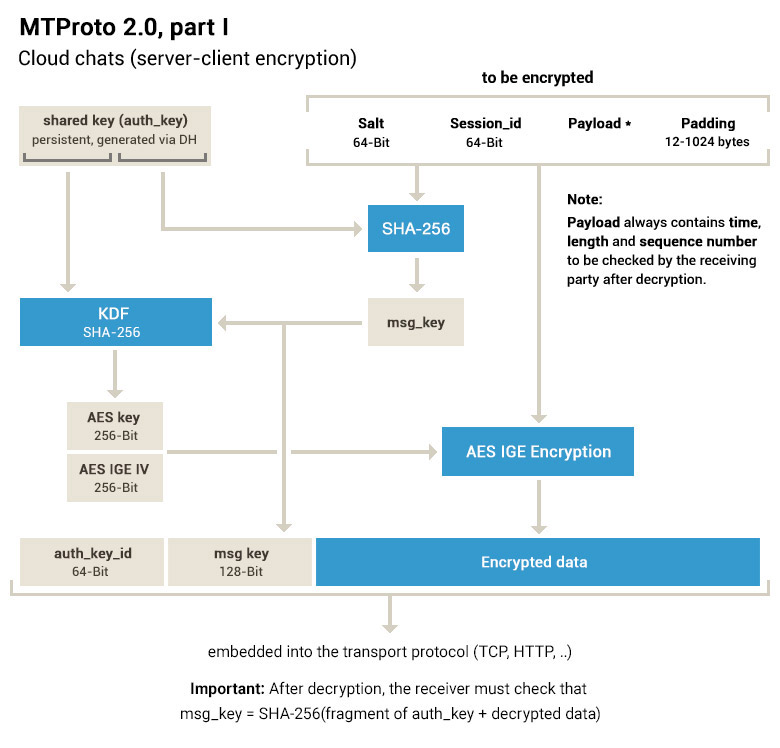
\includegraphics[scale=0.4]{imagenes/diagramaMTProto.jpg} 

\subsection{Resumen de los componentes}
\begin{description}
	\item \textbf{Componentes de alto nivel(Lenguajes de consulta/API RPC):}
Desde el punto de vista del componente de alto nivel, el cliente y el servidor intercambian mensajes dentro de una sesión.\\
La sesión se adjunta al cliente en lugar de una conexión \emph{websocket/http/https/tcp.} 
Además, cada sesión tiene asociada a clave ID de usuario mediante la cual se logra la autorización.\\ 
Pueden estar abiertas varias conexiones a un servidor, los mensajes pueden ser enviados en cualquier dirección a través de cualquiera de las conexiones.
Cuando se usa el protocolo UDP, una respuesta puede ser devuelta por una dirección de IP distinta.\\
Hay diferentes tipos de mensajes:
\begin{itemize}
		\item \textbf{LLamadas RPC(cliente-servidor):} LLamadas a los métodos de la API.
		\item \textbf{Respuestas RPC(servidor-cliente):} Resultados de las llamadas RPC.
		\item \textbf{Notificación del estado de los mensajes}
		\item \textbf{Consultas de estado de mensaje}
		\item \textbf{Mensaje multiparte o contenedor}
\end{itemize}
Desde el punto de vista de protocolos de bajo nivel, un mensaje es un flujo de datos alineados con 4 o 16 bytes de límite.
Los primeros campos en un mensaje están fijos y son usados por el sistema criptográfico o de autorización.\\
Cada mensaje, consiste en un \emph{identificador de mensaje} de 64 bits, \emph{número de secuencia del mensaje dentro de una sesión}, \emph{longitud} de 32 bits y \emph{cuerpo del mensaje} de cualquier tamaño siempre y cuando sea múltiplo de 4. 
Además cuando un contenedor o un mensaje simple se envían, una \emph{cabecera interna} se añade al principio del mensaje, luego el mensaje es cifrado y se le añade una \emph{cabecera externa} la cual será una \emph{clave de identificación} de 64 bits y una \emph{clave del mensaje} de 128 bits.\\
El \emph{cuerpo} del mensaje normalmente consiste en un \emph{tipo mensaje} de 32 bits seguido de los \emph{parámetros dependientes del tipo}.\\
Los números están escritos en \emph{little endian}. Sin embargo los números muy grandes(2048 bits) usados en \textbf{RSA} y \textbf{DH} están escritos en \emph{big endian} porque es lo que hace la biblioteca \textbf{OpenSSL}.
	\item \textbf{Autorización y Cifrado:}
			Antes de que un mensaje sea transmitido por la red usando un protocolo de transporte, este es cifrado añadiendo una cabecera externa la cual es insertada al principio del mensaje y contiene:
	\begin{itemize}
		\item \emph{Identificador de clave} de 64 bits
		\item \emph{Clave de mensaje} de 128 bits
	\end{itemize}
Una clave de usuario junto con una clave de mensaje definen una clave de 256 bits la cual es la que cifra el mensaje usando un cifrado \emph{AES-256}.
La primera parte del mensaje cifrado contiene datos variables(sesión, id del mensaje, número de secuencia) los cuales influyen en la clave del mensaje. La clave del mensaje es definida como los 128 bits iniciales del mensaje cifrado con \emph{SHA-256}, 
además los mensajes en varias partes están cifrados como un solo mensaje.\\
Lo primero que tiene que hacer la aplicación cliente es crear una clave de autorización que se genera normalmente la primera vez que se ejecuta la aplicación y por lo general nunca cambia.\\
Para prevenir potenciales ataques debido a la apropiación de la clave de autorización MTProto soporta \emph{Perfect Forward Secrecy} tanto en los chats en la nube como en los chats secretos.
	\item \textbf{Sincronización de la hora:}
Si la hora de un cliente difiere de la hora del servidor, el servidor podría empezar a ignorar los mensajes de este y recíprocamente el cliente a los mensajes del servidor debido a que el mensaje tenga un indentificador inválido del mensaje.\\
Bajo estas circunstancias, el servidor enviará un mensaje especial al cliente el cual contendrá la hora correcta, este mensaje será el primero en el caso de que también se envíe un grupo de mensajes.\\
Habiendo recibido el mensaje, el cliente primero ejecutará una sincronización de la hora y después verificará el identificador del mensaje para ver si es correcto.\\
En caso de que no sea correcto, el cliente deberá generar una nueva sesión para asegurar la monotonía de los identificadores de los mensajes.
\end{description}
\subsection{Modelo de seguridad}
Los protocolos de Telegram se modelan en ProVerif \cite{ProVer}, que es un verificador criptográfico simbólico. Los protocolos y propiedades de seguridad están especificadas en una variante del \emph{$\pi$-cálculo} que es una notación desarrollada por Robin Milner, Joachim Parrow y David Walker, como un avance sobre el cálculo de sistemas comunicantes con el fin de proveer movilidad al modelado concurrente para representar procesos criptográficos y traducirlos en una teoría de Horn.\\
MTProto 2.0 sigue la siguiente regla de reducción

\lstinputlisting[
    caption=Regla Reducción 1,
    label={lst:listing-cpp},
    language=C++,
    style=CodigoC,
    ]{./ejemplos/ejemplo1.cpp}

%\subsection{Protocolo MTProto 2.0}
%Como se ha mencionado anteriormente MTProto es una suite cliente/servidor diseñada para acceder a servidores MTProto. Esta suite se puede dividir tres componentes principales.

%\begin{itemize}
	%\item \textbf{API de alto nivel:} Define como las consultas de la API y respuestas de esta son convertidas en mensajes binarios.
	%\item \textbf{Componentes criptográficos y de autorización:} Definen como la aplicaciones se autentifican con el servidor y los mensajes son cifrados antes de ser transmitidos a través del protocolo de transporte.	
	%\item \textbf{Componente de transporte:} Define como el cliente y el servidor realmente intercambian los mensajes por un protocolo existente como UDP, TCP, HTTP, HTTPS, etc. Cabe a destacar que también los protocolos de conexión inseguros son soportados.
	%\item \textbf{Autorización:} Este módulo provee las funcionalidades para la primera autorización del cliente y del servidor. Se ejecuta solo en la primera ejecución de la aplicación.
%\end{itemize}
%\\
